Occupancies close to the beam create many of the key challenges in the HPS experiment
and determine the limits of sensitivity a low A$^\prime$ masses.
These occupancies are dominated by electrons scattered to large angles 
in the target. Because HPS is sensitive to scattering angles very far out 
on the tail, beyond angles important in other experiments, care must be taken
to ensure our simulations are correct in this regime.  In particular,
Geant4 overestimates the multiple scattering rate by a factor of 2 (see Figure \ref{fig:egs_geant}) at large angles. 
One of the main goals of the test run in 2012 was to evaluate the description of the tails of the multiple scattering in order 
to gain further confidence in our expected detector occupancy. As will be shown below, data from the 
test run can be used to confirm our model of multiple coulomb scattering despite the fact that 
all data was taken with a photon beam.

%\begin{figure*}[t]
%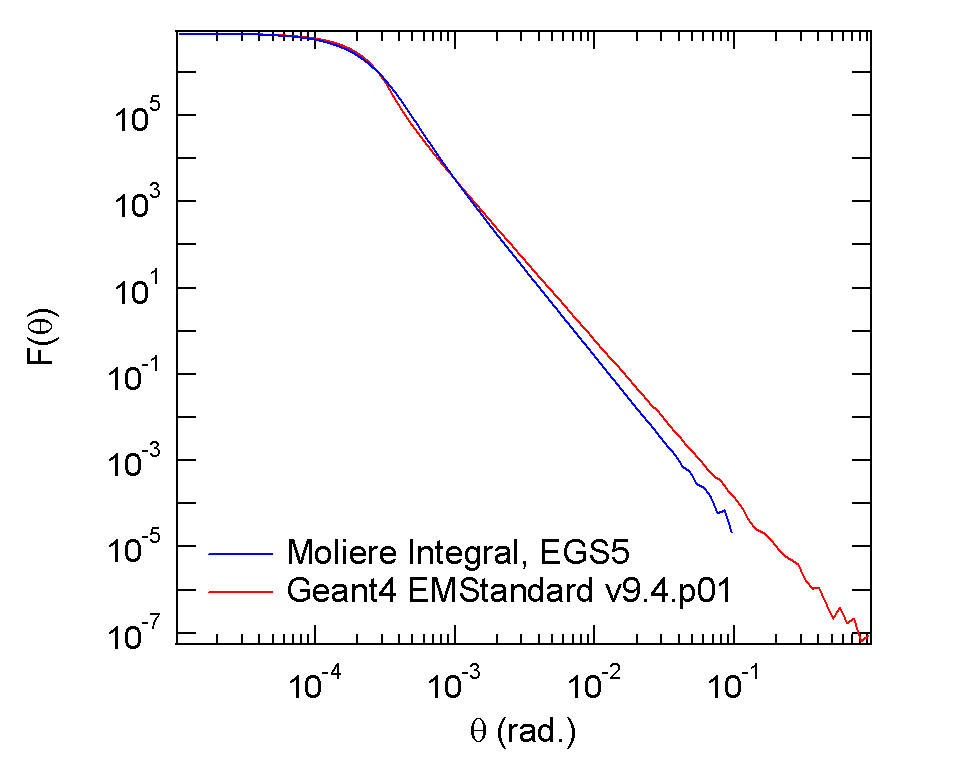
\includegraphics[ scale=0.7]{test2012/angular_measurement/pictures/egs_geant}
%\caption{\small{Comparison of EGS5 and Geant4 multiple scattering cross-sections.}}\label{fig:egs_geant}
%\end{figure*}

Figure~\ref{fig:schematic_testrun_vs_erun} gives a schematic view of the main differences 
between the photon and electron beam setup. 
\begin{figure*}[t]
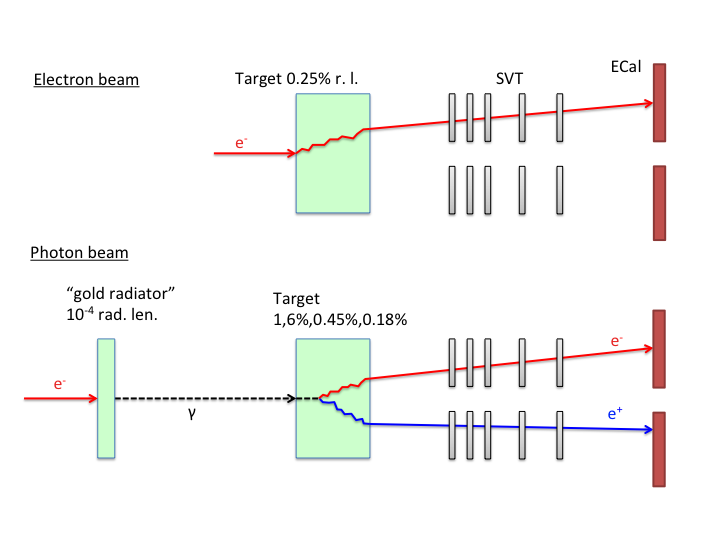
\includegraphics[ scale=0.5]{test2012/angular_measurement/pictures/photon_vs_electron_beam_schematic.png}
\caption{\small{Schematic comparison of the photon beam setup to the electron beam.}}\label{fig:schematic_testrun_vs_erun}
\end{figure*}
In particular, the angular distribution of the pair produced electron and positions emerging 
from the target has contributions from two sources: {\it i} the pair production angle $\alpha$ 
and {\it ii} the resulting angle from multiple scattering in the target after production. This is 
schematically described in Fig.~\ref{fig:schematic_pair_prod}. 
\begin{figure*}[t]
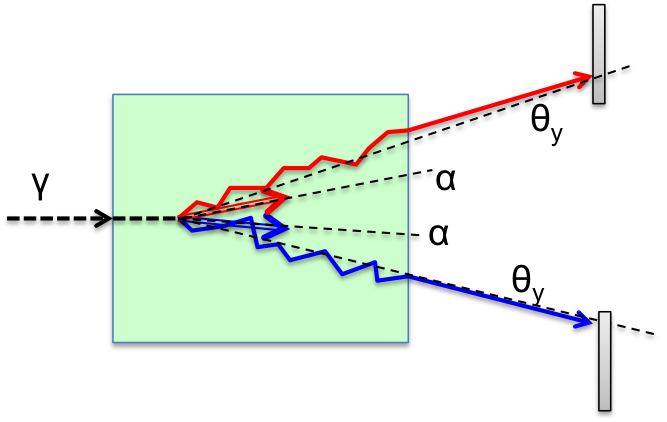
\includegraphics[ scale=0.7]{test2012/angular_measurement/pictures/pair_prod_schematics.png}
\caption{\small{Schematic description of the relevant angles for pair production in the 
test run.}}\label{fig:schematic_pair_prod}
\end{figure*}
The contribution from both sources to the final angular distribution are comparable. 
%FigureX 
%shows the expected distribution of the vertical angle $\theta_y$ for the $e^+e^-$ pair  coming 
%out of the converter compared to the pair production angle. {\color{red} Need this figure from Takashi.} 


%{\bf Sample Composition}\newline

Since we are primarily interested in measuring the angular 
distributions for the $e^+e^-$ pair we checked that the contribution from photons in our triggered sample are negligible. Table~\ref{tab:sample_composition} shows the sample composition. The fraction of photons that would deposit energy to reach threshold in the ECal crystals are much less than 2\% without any angular selection which will further reduce the fraction of photons. 
\begin{table}[]
\centering
\begin{tabular}{c|c|c|c}
Type & Nominal & $E>0.2$~GeV & $E>0.5$~GeV \\
\hline
electron & 7150 & 4938 & 3186 \\
positron & 6019 & 4568 & 2874 \\
$e^+e^-$ & 13169 & 9506 & 6060 \\
photon & 2984 & 640 & 151 \\
\hline
\end{tabular}
\caption{Sample composition for the photon test run.}
\label{tab:sample_composition}
\end{table}

The photon beam line during the test run produced a relatively large fraction of pairs 
originating upstream of the converter. This contribution was measured during data taking by 
removing the converter and thus taking data without any target but with all other conditions 
the same. Figure~\ref{fig:extrapol_converter} (bottom) shows the vertical position of 
reconstructed tracks in the SVT during data taking with a converter thickness of 
1.6\% radiation length. Note the small satellite peaks visible at about $\pm 10$~mm which 
can be identified as the upstream background when studying the same distribution from the 
run without any converter. 
%\begin{figure*}[t]
%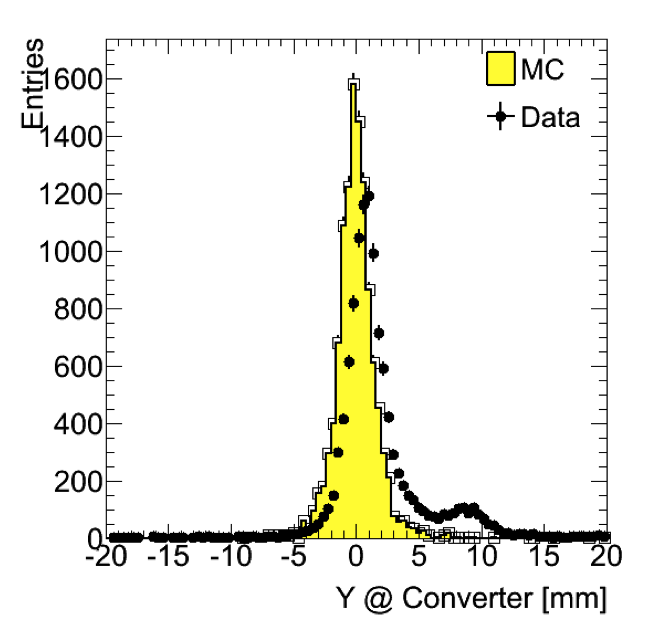
\includegraphics[ scale=0.6]{test2012/angular_measurement/pictures/tracks_at_converter_Y_top.png}
%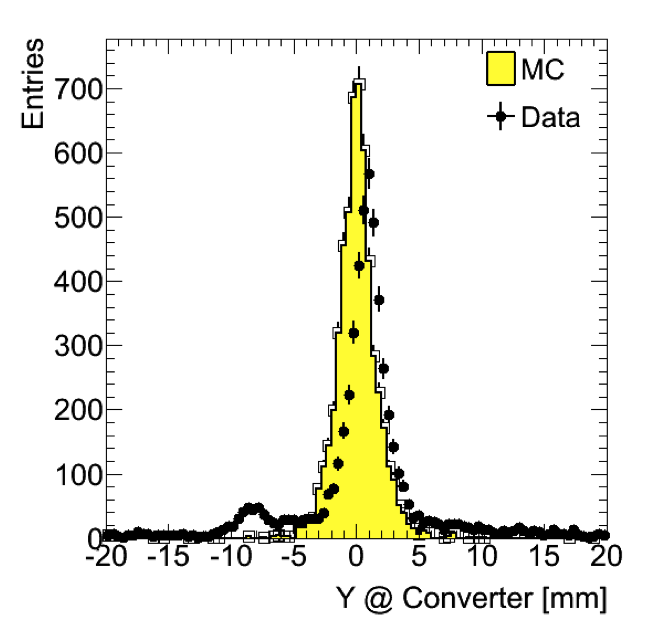
\includegraphics[ scale=0.6]{test2012/angular_measurement/pictures/tracks_at_converter_Y_bottom.png}
%\caption{\small{Vertical position of extrapolated tracks from the SVT to the converter position.} {\color{red}Need update.}}\label{fig:tracks_at_converter}
%\end{figure*}

In order to properly normalize the rates the integrated current was measured for the different 
runs. Typically the current was about 30~nA. Table.~\ref{tab:currents} shows the measured integrated currents.  The uncertainty of the measurement is estimated to be approximately 5\%. 
\begin{table}
\centering
\begin{tabular}{l|c|c|c}
%Run & Target thickness [\%r.l.] &   start time[s]      & end time [s] & Duration [s] &       integrated beam current (nC)    \\                thickness (%r.l.)       Rate(Hz)     Recorded(Hz)  Magnet Polarity
Run & Target thickness & Duration &  $e^-$ on converter \\
 &  (\%r.l.) & (s) & (nC)    \\   
\hline\hline
1351 & 1.6   & 911 &     24385.9     \\
\hline
1353 & 0.18   & 2640 &    193508.9  \\
\hline
1354 & 0.45  & 2149 &       140709.9  \\
\hline
1358 & 0    & 1279  &   88079.6  \\
%1349    1337323714      1337324625      51344.0926551819        54879.7343788147        1.6                     1262.120     1174.728      -1
%1351    1337324962      1337325268      24385.9185791016        26928.0426635742        1.6                     1933.479     1696.808      -1
%1353    1337325717      1337328357      193508.881838322        204325.132622242        0.18                    436.895      425.659       -1
%1354    1337328521      1337330670      140709.898532331        148839.141475141        0.45                    596.055      570.870       -1
%1358    1337331152      1337332431      88079.5567516331        92523.9428218845        0                       309.785      304.253       -1
%1359    1337332615      1337334014      91653.0026320741        91761.4541434497        0                       318.640      311.540       1
%1360    1337334136      1337336898      198670.590789914        209883.979889035        0.18                    451.067      446.510       1
%1362    1337337264      1337338713      105642.70688653         110298.553449392        1.6                     1864.090     1659.675      1
%1363    1337340178      1337340456      8556.8459701538         8556.8459701538         1.6                     1864.090     1659.675      1
\hline
\end{tabular}
\caption{{\small Measured integrated currents for the runs used to measure the angular distributions.}}
\end{table}
Taking into account the measured integrated current 
the upstream background fraction was 16\%, 52\% and 71\% 
for converter thicknesses of 1.6\%, 0.45\% and 0.18\%, respectively. 

The measured angular distribution in the ECal for the three target thicknesses are shown in 
Fig.~\ref{fig:ang_distr_data} before and after normalization and subtraction of the upstream 
background contribution.
\begin{figure*}[t]
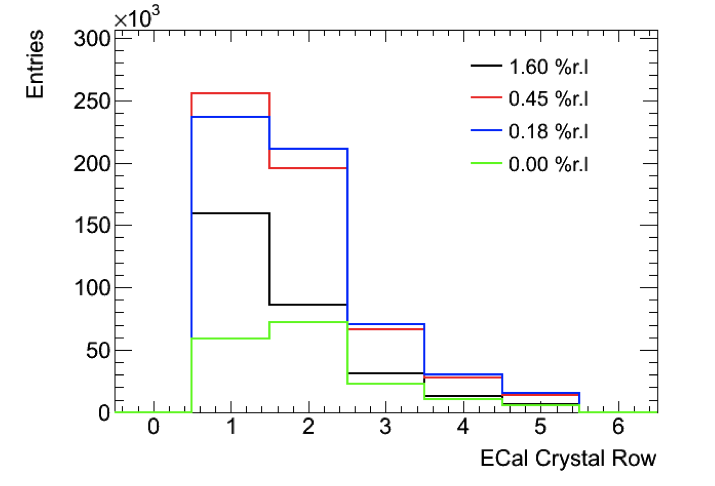
\includegraphics[ scale=0.65]{test2012/angular_measurement/pictures/rate_ecalrow_raw.png}
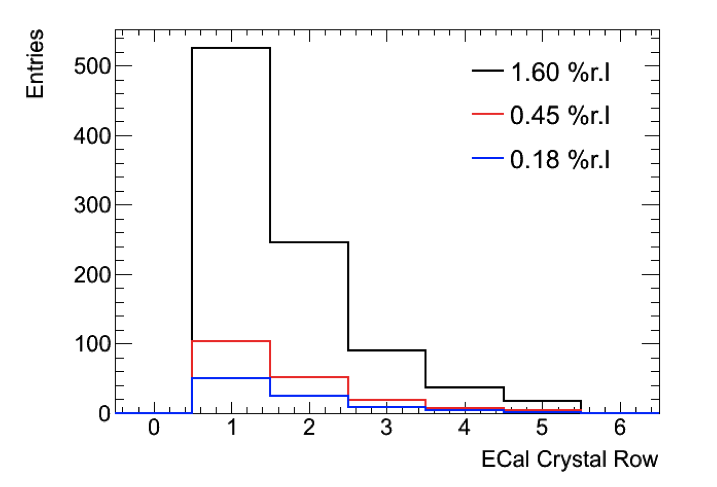
\includegraphics[ scale=0.65]{test2012/angular_measurement/pictures/rate_ecalrow_norm_subtr.png}
\caption{\small{Measured raw vertical angular distributions before (left) and after (right) 
normalization and background subtraction.} {\color{red} Need update.}}
\label{fig:ang_distr_data}
\end{figure*}

These measured angular distributions are then compared to simulation. 
While the bulk of multiple coulomb scattering and pair production angles 
are well studied in the past {\color{red} (references?)} HPS 
is sensitive only to the large part of these distributions that are less explored. 
Note that for HPS we are only interested in validating our description of the multiple coulomb scattering, as that 
is our main background when running in an electron beam. Since 
what we measure in ~\ref{fig:ang_distr_data} is a convolution of both we use a special event 
generation procedure in the simulation to separate description of the multiple scattering and 
pair production angle: we use EGS5~\cite{egs5} to generate the pair produced $e^+e^-$ pair 
and then pass these four vectors to either {\sc EGS5} or {\sc Geant4}~\cite{geant4} which 
models the multiple Coulomb scattering in the target. Thus the {\sc EGS5} is used to normalize 
the pair production angles and the remaining difference would be coming from the 
multiple scattering description in the two different simulation programs. There exist an unlikely 
scenario that the difference in multiple scattering between the two programs would cancel the difference in multiple scattering. To mitigate this possibility the angular distributions are 
measured for different converter thickness. Since the pair production angle is independent of 
the converter thickness the relative change between data and simulation for different converter thicknesses only depends on the multiple scattering contribution. 

Figure~\ref{fig:ang_distr_dataMC} shows a comparison between data and the {\sc EGS5} 
simulation where the rates have been normalized to 1~s of beam at a current of 90nA. 
\begin{figure*}[t]
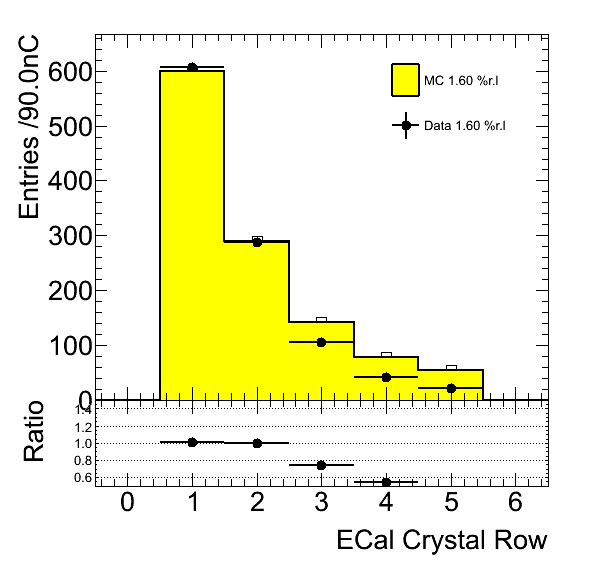
\includegraphics[ scale=0.25]{test2012/angular_measurement/pictures/dataMC_1351_Hit_Y_top_norm_bkgsub.png}
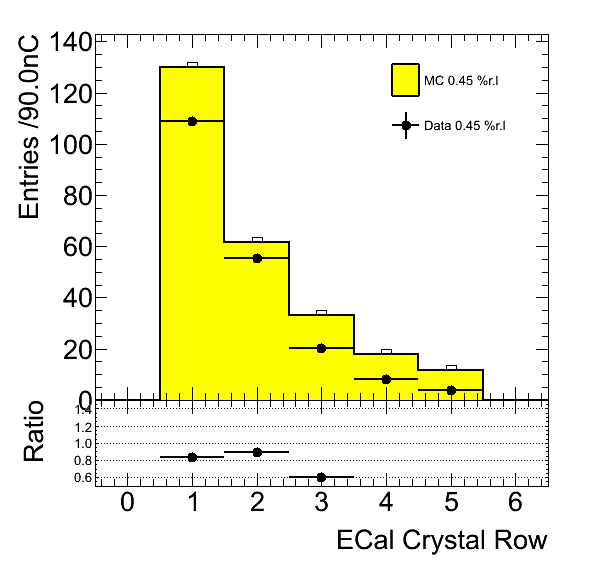
\includegraphics[ scale=0.25]{test2012/angular_measurement/pictures/dataMC_1354_Hit_Y_top_norm_bkgsub.png}
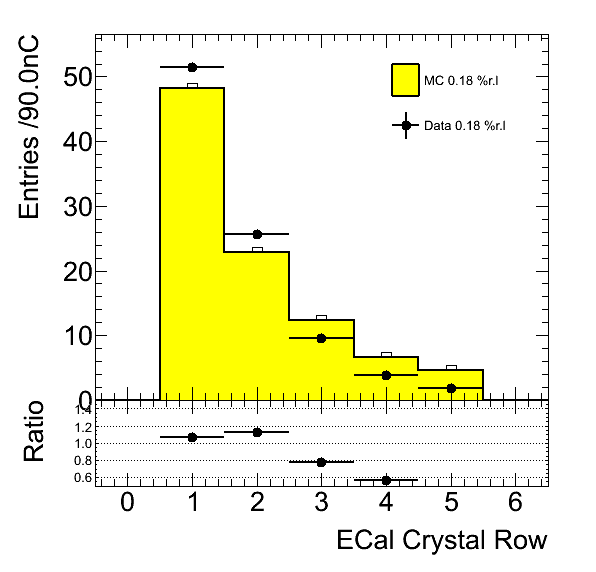
\includegraphics[ scale=0.25]{test2012/angular_measurement/pictures/dataMC_1353_Hit_Y_top_norm_bkgsub.png}
\caption{\small{Comparison between the observed and simulated angular 
distribution using {\sc EGS5} for a converter thickness of 1.6\% (left), 0.45\% (middle) and 0.18\% 
(right).  Only statistical uncertainties are included. }}
\label{fig:ang_distr_dataMC}
\end{figure*}
The total rate prediction for simulation and data are compared in Fig.~\ref{rate_vs_thickness} 
and Tab.~\ref{tab:ang_distr_dataMC} summarizes the result. 
\begin{figure*}[t]
%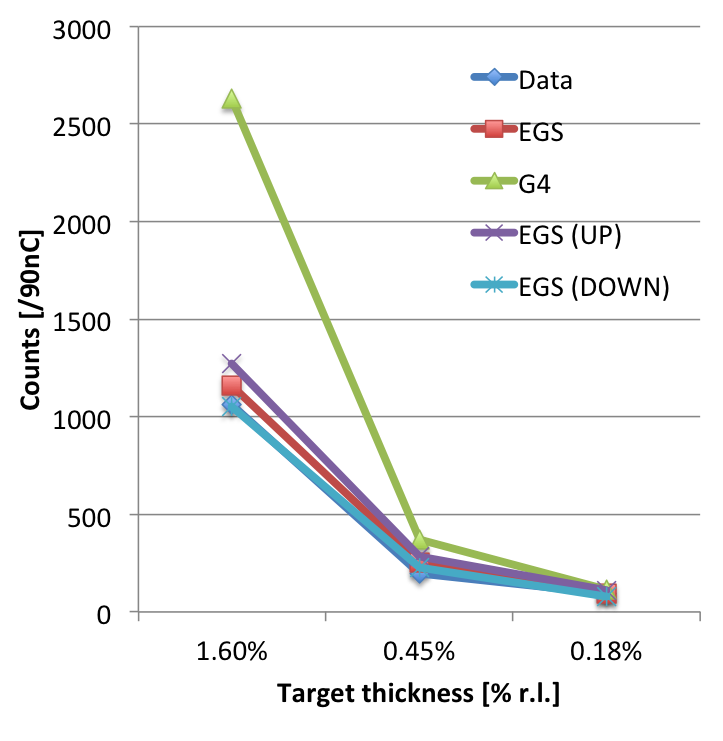
\includegraphics[ scale=0.65]{test2012/angular_measurement/pictures/rate_vs_thickness_dataMC.png}
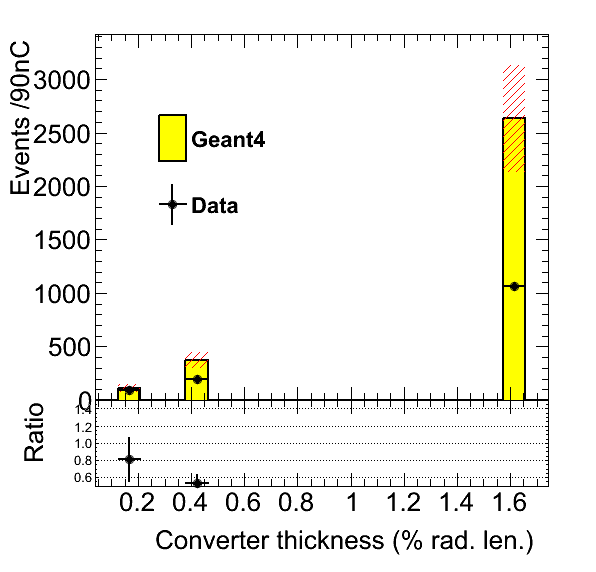
\includegraphics[ scale=0.3]{test2012/angular_measurement/pictures/dataMC_geant4.png}
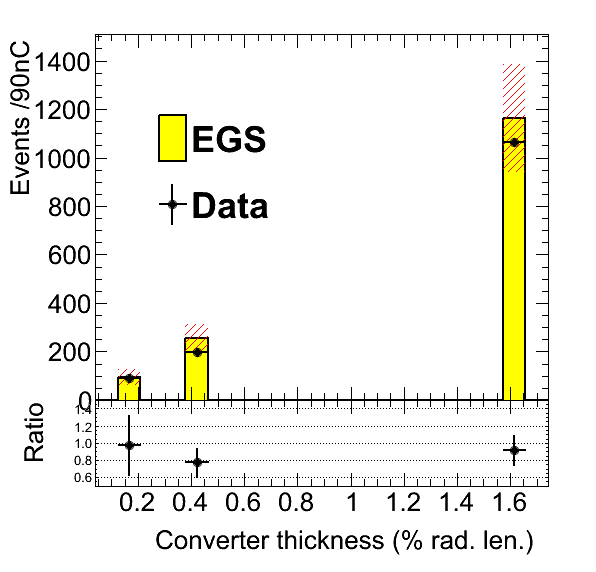
\includegraphics[ scale=0.3]{test2012/angular_measurement/pictures/dataMC_egs.png}
\caption{\small{The measured rate in the ECal as a function of target thickness comparing 
to the multiple scattering models from {\sc Geant4} (left) and {\sc EGS5} (right)}.} 
\label{fig:rate_vs_thickness}
\end{figure*}
A few systematic uncertainties was estimated which include; a 5\% uncertainty on the integrated 
current normalization, limited Monte Carlo statistics, alignment of the ECal and uncertainty 
from the background normalization. 
%The uncertainty from the initial gain calibration of the 
%ECal described in Sec.{\color{red} X} was estimated to be less than {\color{red} Y\%, need to check this %calibration systematic.}.
\begin{table}
\begin{tabular}{|l|c|c|c|}
\hline
Converter (\% r.l.) & 1.60 & 0.45 &	0.18 \\
\hline
{\sc EGS5} &	1162 $\pm$ 112 &	255 $\pm$ 28 &	94 $\pm$ 17	\\
\hline
{\sc Geant4} & 2633 $\pm$ 250 & 	371 $\pm$ 38 &	114 $\pm$ 18 \\
\hline
Observed 	& 1064 $\pm$ 2 & 196 $\pm$ 1 &	92 $\pm$ 1 \\						
%Beam gap	58	13	5	132	19	6
%	EGS			G4		
%Target thickness	1.60%	0.45%	0.18%	1.60%	0.45%	0.18%
%Data [/90nC]	1064	196	92	1064	196	92
%Pred. [/90nC]	1162	255	94	2633	371	114
%Total uncertainty	112	28	17	250	38	18
%Stat	2	1	1	2	1	1
%						
%Stat MC	11	3	1	16	3	1
%Bkg norm.	14	14	14	14	14	14
%Current norm.	94	21	8	212	30	9
%Beam gap	58	13	5	132	19	6
\hline
\end{tabular}
\caption{ {\small Observed and predicted events for 1~s of beam at 90nA for different converter 
thicknesses. The uncertainty on the predictions is the total uncertainty including estimated 
systematic uncertainties. }}
\end{table}
With the set of conservative systematics the total systematic uncertainty was between 10 and 18\%. 

In summary, it is clear that the version of  
{\sc Geant4} with the default physics lists overestimates the large angle multiple scattering tail. 
Since {\sc EGS5} was used to generate the pair 
angle distribution for both simulation described in the result it's interesting to see that the 
ratio of data to the prediction varied from 0.91 (0.40), 0.77 (0.53) and 0.98 (0.81) for {\sc EGS} 
({\sc Geant4}) at 1.6\%, 0.45\% and 0.18\% converter thickness, respectively. If the pair angle 
distribution were responsible for the difference between {\sc Geant4}  and {\sc EGS5} that would show up as a large shift in this ratio since the multiple scattering contribution varies. 

There are more work needed to go from this preliminary result to a real 
measurement. However, this preliminary result further strengthens our confidence that 
{\sc EGS5} is able to properly describe the large angle multiple scattering events in the target 
which is important to estimate our occupancy and trigger rates for HPS (see Sec.~\ref{sec:performance}).
